\documentclass[portrait,final,a0paper]{baposter}
%\documentclass[a4shrink,portrait,final]{baposter}
% Usa a4shrink for an a4 sized paper.

\tracingstats=2

\usepackage{calc}
\usepackage{graphicx}
\usepackage{amsmath}
\usepackage{amssymb}
\usepackage{relsize}
\usepackage{multirow}
\usepackage{bm}
\usepackage{graphicx}
\usepackage{multicol}
\usepackage{ marvosym }
\usepackage[utf8]{inputenc}
\DeclareUnicodeCharacter{00A0}{ }
\usepackage{pgfbaselayers}
\pgfdeclarelayer{background}
\pgfdeclarelayer{foreground}
\pgfsetlayers{background,main,foreground}
\usepackage[francais]{babel}
\usepackage{times}
\usepackage{helvet}
%\usepackage{bookman}
\usepackage{palatino}

\newcommand{\captionfont}{\footnotesize}

\selectcolormodel{cmyk}

\graphicspath{{images/}}

%%%%%%%%%%%%%%%%%%%%%%%%%%%%%%%%%%%%%%%%%%%%%%%%%%%%%%%%%%%%%%%%%%%%%%%%%%%%%%%%
%%%% Some math symbols used in the text
%%%%%%%%%%%%%%%%%%%%%%%%%%%%%%%%%%%%%%%%%%%%%%%%%%%%%%%%%%%%%%%%%%%%%%%%%%%%%%%%
% Format 
\newcommand{\Matrix}[1]{\begin{bmatrix} #1 \end{bmatrix}}
\newcommand{\Vector}[1]{\Matrix{#1}}
\newcommand*{\SET}[1]  {\ensuremath{\mathcal{#1}}}
\newcommand*{\MAT}[1]  {\ensuremath{\mathbf{#1}}}
\newcommand*{\VEC}[1]  {\ensuremath{\bm{#1}}}
\newcommand*{\CONST}[1]{\ensuremath{\mathit{#1}}}
\newcommand*{\norm}[1]{\mathopen\| #1 \mathclose\|}% use instead of $\|x\|$
\newcommand*{\abs}[1]{\mathopen| #1 \mathclose|}% use instead of $\|x\|$
\newcommand*{\absLR}[1]{\left| #1 \right|}% use instead of $\|x\|$

\def\norm#1{\mathopen\| #1 \mathclose\|}% use instead of $\|x\|$
\newcommand{\normLR}[1]{\left\| #1 \right\|}% use instead of $\|x\|$

%%%%%%%%%%%%%%%%%%%%%%%%%%%%%%%%%%%%%%%%%%%%%%%%%%%%%%%%%%%%%%%%%%%%%%%%%%%%%%%%
% Multicol Settings
%%%%%%%%%%%%%%%%%%%%%%%%%%%%%%%%%%%%%%%%%%%%%%%%%%%%%%%%%%%%%%%%%%%%%%%%%%%%%%%%
\setlength{\columnsep}{0.7em}
\setlength{\columnseprule}{0mm}


%%%%%%%%%%%%%%%%%%%%%%%%%%%%%%%%%%%%%%%%%%%%%%%%%%%%%%%%%%%%%%%%%%%%%%%%%%%%%%%%
% Save space in lists. Use this after the opening of the list
%%%%%%%%%%%%%%%%%%%%%%%%%%%%%%%%%%%%%%%%%%%%%%%%%%%%%%%%%%%%%%%%%%%%%%%%%%%%%%%%
\newcommand{\compresslist}{%
\setlength{\itemsep}{1pt}%
\setlength{\parskip}{0pt}%
\setlength{\parsep}{0pt}%
}


%%%%%%%%%%%%%%%%%%%%%%%%%%%%%%%%%%%%%%%%%%%%%%%%%%%%%%%%%%%%%%%%%%%%%%%%%%%%%%
%%% Begin of Document
%%%%%%%%%%%%%%%%%%%%%%%%%%%%%%%%%%%%%%%%%%%%%%%%%%%%%%%%%%%%%%%%%%%%%%%%%%%%%%

\begin{document}

%%%%%%%%%%%%%%%%%%%%%%%%%%%%%%%%%%%%%%%%%%%%%%%%%%%%%%%%%%%%%%%%%%%%%%%%%%%%%%
%%% Here starts the poster
%%%---------------------------------------------------------------------------
%%% Format it to your taste with the options
%%%%%%%%%%%%%%%%%%%%%%%%%%%%%%%%%%%%%%%%%%%%%%%%%%%%%%%%%%%%%%%%%%%%%%%%%%%%%%
% Define some colors
\definecolor{silver}{cmyk}{0,0,0,0.3}
\definecolor{yellow}{cmyk}{0,0,0.9,0.0}
\definecolor{reddishyellow}{cmyk}{0,0.22,1.0,0.0}
\definecolor{black}{cmyk}{0,0,0.0,1.0}
\definecolor{darkYellow}{cmyk}{0,0,1.0,0.5}
\definecolor{darkSilver}{cmyk}{0,0,0,0.1}

\definecolor{lightyellow}{cmyk}{0,0,0.3,0.0}
\definecolor{lighteryellow}{cmyk}{0,0,0.1,0.0}
\definecolor{lighteryellow}{cmyk}{0,0,0.1,0.0}
\definecolor{lightestyellow}{cmyk}{0,0,0.05,0.0}

%%
\typeout{Poster Starts}
\background{
  \begin{tikzpicture}[remember picture,overlay]%
    \draw (current page.north west)+(-2em,2em) node[anchor=north west] {\includegraphics[height=1.1\textheight]{silhouettes_background}};
  \end{tikzpicture}%
}

\newlength{\leftimgwidth}
\begin{poster}%
  % Poster Options
  {
  % Show grid to help with alignment
  grid=false,
  % Column spacing
  colspacing=1em,
  % Color style
  bgColorOne=lighteryellow,
  bgColorTwo=lightestyellow,
  borderColor=reddishyellow,
  headerColorOne=yellow,
  headerColorTwo=reddishyellow,
  headerFontColor=black,
  boxColorOne=lightyellow,
  boxColorTwo=lighteryellow,
  % Format of textbox
  textborder=roundedleft,
%  textborder=rectangle,
  % Format of text header
  eyecatcher=true,
  headerborder=open,
  headerheight=0.08\textheight,
  headershape=roundedright,
  headershade=plain,
  headerfont=\Large\textsf, %Sans Serif
  boxshade=plain,
%  background=shade-tb,
  background=plain,
  linewidth=2pt
  }
  % Eye Catcher
  {
\includegraphics[width=10em]{docknroll}} % No eye catcher for this poster. (eyecatcher=no above). If an eye catcher is present, the title is centered between eye-catcher and logo.
  % Title
  {\sf %Sans Serif
  %\bf% Serif
   Développer, Tester et Livrer des \mbox{Microservices à l'aide de Docker}}
  % Authors
  {\sf %Sans Serif
  % Serif
  \vspace{0.5em}
  Nicolas Herbaut (LaBRI, ENSEIRB-MATMECA) \mbox{David Bourasseau et Maxime Peterlin (ENSEIRB-MATMECA)}
  }
  % University logo
  {% The makebox allows the title to flow into the logo, this is a hack because of the L shaped logo.
    \makebox[8em][r]{%
      \begin{minipage}{16em}
        \hfill
        \begin{flushright}
	        
		
		
\includegraphics[height=4em]{labri}
        
\includegraphics[height=4em]{enseirb-matmeca}\\
        
\includegraphics[height=3em]{jdevlogo2015.png}
		\end{flushright}
      \end{minipage}
    }
    
    
  }

  \tikzstyle{light shaded}=[top color=baposterBGtwo!30!white,bottom color=baposterBGone!30!white,shading=axis,shading angle=30]

  % Width of left inset image
     \setlength{\leftimgwidth}{0.78em+8.0em}

%%%%%%%%%%%%%%%%%%%%%%%%%%%%%%%%%%%%%%%%%%%%%%%%%%%%%%%%%%%%%%%%%%%%%%%%%%%%%%
%%% Now define the boxes that make up the poster
%%%---------------------------------------------------------------------------
%%% Each box has a name and can be placed absolutely or relatively.
%%% The only inconvenience is that you can only specify a relative position 
%%% towards an already declared box. So if you have a box attached to the 
%%% bottom, one to the top and a third one which should be in between, you 
%%% have to specify the top and bottom boxes before you specify the middle 
%%% box.
%%%%%%%%%%%%%%%%%%%%%%%%%%%%%%%%%%%%%%%%%%%%%%%%%%%%%%%%%%%%%%%%%%%%%%%%%%%%%%
    %
    % A coloured circle useful as a bullet with an adjustably strong filling
    \newcommand{\colouredcircle}[1]{%
      \tikz{\useasboundingbox (-0.2em,-0.32em) rectangle(0.2em,0.32em); \draw[draw=black,fill=baposterBGone!80!black!#1!white,line width=0.03em] (0,0) circle(0.18em);}}


  \headerbox{Contribution}{name=contribution,column=0,row=0}{
  \vspace{0.3em}
  
   Nous exposons un \textbf{retour d'expérience} sur le déroulé de 2 projets étudiants où nous avons utilisé Docker au service d'une architecture Microservice.
   
   Nous expliquons comment nous avons utilisé Docker comme \textbf{unité de déploiement} pour les mises en production et comme \textbf{unité de développement} pour les tests et l'Intégration Continue.
   
   \vspace{1em}
   \textbf{Mots clés}: \textit{Docker, Architecture Microservice, Architecture RestFul, Intégration Continue, Jenkins, Tests Unitaires, Tests d'intégration, Java, Mock.}


 }
   \headerbox{Cobaye: Le Projet SnapMail}{name=project,column=1,span=2,row=0}{

   \begin{multicols}{2}
	   
			
			\begin{minipage}{0.5\textwidth}
			\vspace{1em}
				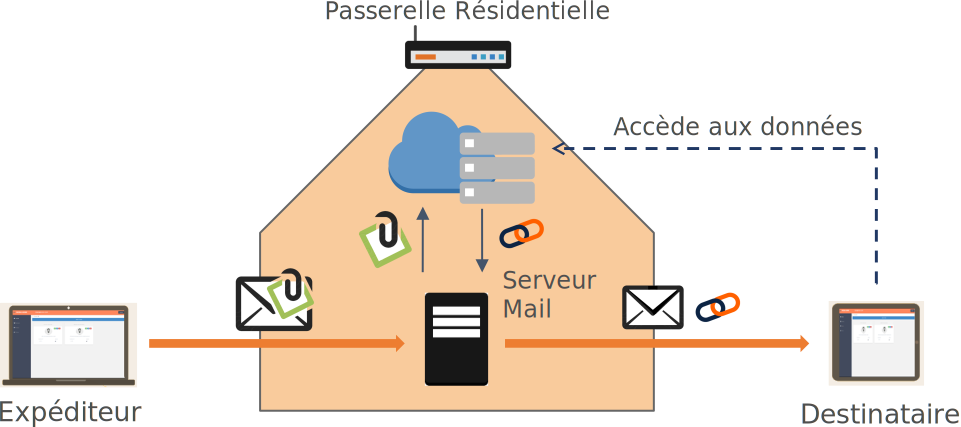
\includegraphics[width=\textwidth]{snapmail}
				\begin{center}\textbf{Plateforme privée d'hébergement de pièces jointes}
				
				\end{center}
				
			\end{minipage}
			
				
			
			Pour pallier au problème des \textbf{pièces jointes volumineuses}, un server SMTP est déployé sur une passerelle résidentielle.
			L'utilisateur configure son client mail avec ce server afin d'y faire transiter son courrier sortant. 
			La passerelle va \textbf{détacher les pièces jointes}, \textbf{les stocker} et \textbf{les remplacer par des liens} dans le mail . Ces liens pointent vers les contenus originaux ainsi que vers des \textbf{versions optimisées} des videos (streaming adaptatif) et photos (converties et redimentionnées).
			
			Le projet est conçu comme un greffon à un autre projet de \textbf{réseau social distribué } également déployé sur les passerelles résidentielles.
			
			
	\end{multicols}
    }
 
   \headerbox{Bénéfices des Microservices}{name=microdesc,column=0,row=0,below=contribution}{
   
  
  
  \begin{center}
   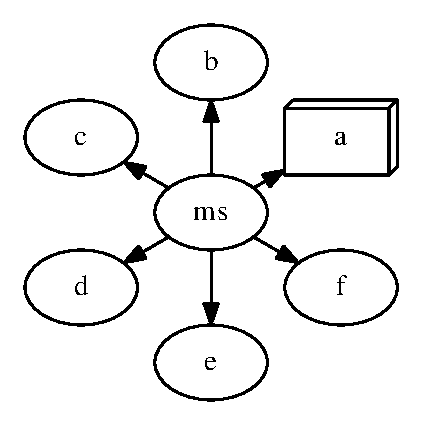
\includegraphics[width=\textwidth]{msprinciples}
   \textbf{Principes guidant les architectures Microservices.}
   \end{center}
   
   Les MS sont des \textbf{Services petits et autonomes qui fonctionnent ensembles}, promouvant un couplage lâche et une cohésion forte.
   Les MS émergent des tendances actuelles de l'ingénieurie logicielle (\textit{Design Driven Development, Livraison Continue, Virtualisation, Agilité, mouvement DevOps, Antifragile}) etc.
   
   
   
	


 }
   \headerbox{Mise en place dans nos projets}{name=micro,column=1,span=2,row=0,below=project}{
   \vspace{2em}
   \begin{multicols}{2}
		   \begin{minipage}{0.5\textwidth}
						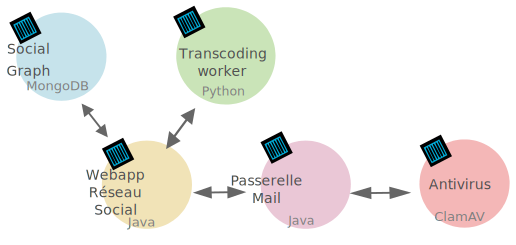
\includegraphics[width=\textwidth]{snapservices}
						\begin{center}\textbf{Découpage selon les concepts métiers}
						\vspace{2em}
						\end{center}
					\end{minipage}
					
	
	Les domaines sont suffisament différents pour que les contours métiers soient clairs: \textit{Réseau Social, Transcoding Multimédia, Email, Antivirus}. Nous choisissons de passer sous une architecture Microservices (MS) pour plusieurs raisons:
	\vspace{1em}
	\begin{itemize}
		\item Les deux projets doivent être évalués indépendamment sans que l'un compromette l'autre. \MVRightarrow \  \textbf{séparation des dépots de sources, pas de code partagé, pas de base de données commune}.
		\item Communication nécessaire entre services \MVRightarrow \ \textbf{Mise en place de l'API REST}.
		\item Choix du meilleur langage pour chaque service (Java, Python) \MVRightarrow \ \textbf{Hétérogénéité des solutions techniques masquée derrière l'API}.
		\item Nécessité de faire tourner les autres services en local pour développer le sien\MVRightarrow \ \textbf{Dockerisation des MS, déploiement des MS pré-configurés dans DockerHub, récupération automatique des images par le dev}.
		\item Approche agile du développement entrainant une démo du produit global tous les 15 jours \MVRightarrow \ \textbf{déploiement de toute la solution avec Docker Compose en pré-prod. La livraison d'un service défectueux peut être reportée}.
		
	\end{itemize} 
	
					
	\end{multicols}
	
   \vspace{1.8em}
 }
 
   \headerbox{Typologie des tests}{name=cidesc,column=0,row=0,below=microdesc}{
  
  
   \begin{center}
	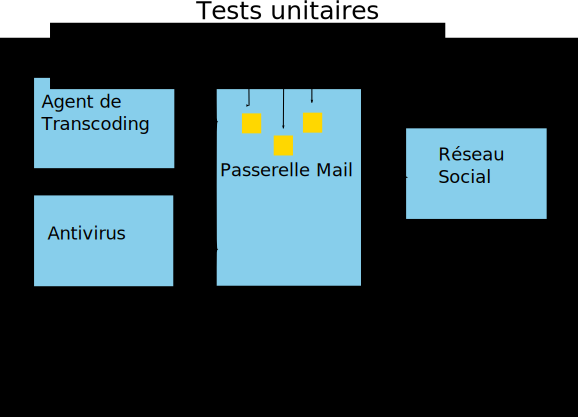
\includegraphics[width=\textwidth]{tests}
    \textbf{Trois niveaux de tests automatisés dans une architecture Microservices}
   \end{center}
   
   
   

   
 }
   \headerbox{Intégration Continue \& workflow de développement}{name=ci,column=1,span=2,row=0,below=micro}{
   
	\begin{center}
	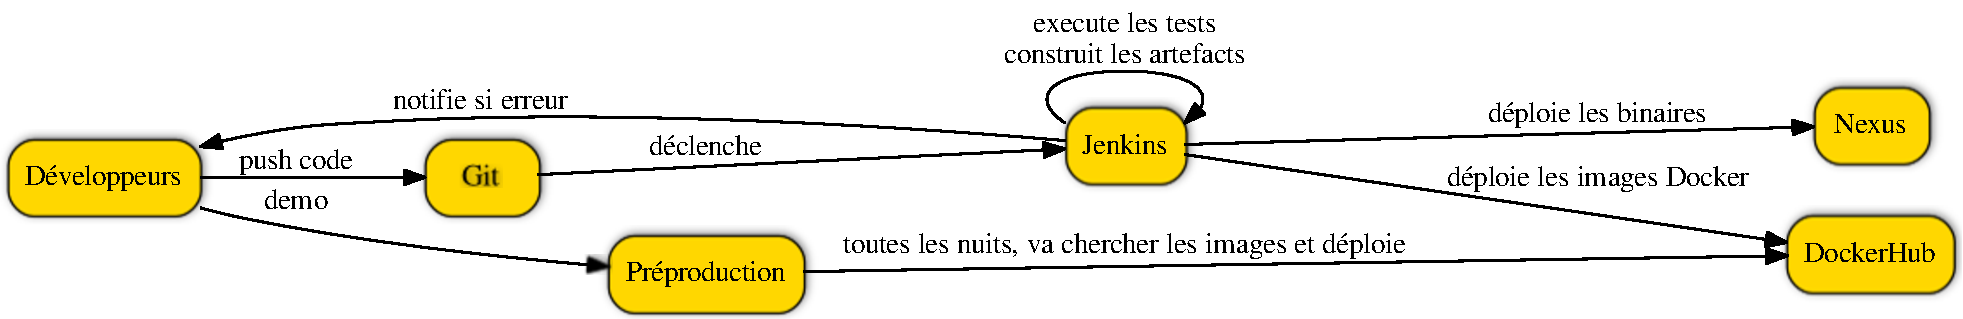
\includegraphics[width=\textwidth]{workflow}
    \textbf{Workflow de développement}
   
   \end{center}
    \begin{multicols}{2}
    
Tester une architecture Microservice montre certaines particularités par rapport aux monolithes.
\begin{itemize}
	\item En raison de l'homogénéité du métier, \textbf{les tests unitaires} sont plus simples à écrire. 
	\item  \textbf{Les tests de services} nécessitent l'utilisation de mocks d'interfaces REST, que nous avons réalisé avec Montbank (http://www.mbtest.org/).
	\item Une fois par jour, Jenkins réalise une série de \textbf{tests de bout en bout} en lançant un environnement iso-production des services et en faisant jouer des scénarios utilisateurs.
	\item Grace au DockerHub, toutes les machines autorisées peuvent récupérer les images docker et les lancer à tout moment. Les \textbf{bugs sont donc plus facilement reproduits} sur la machine du développeur.
\end{itemize}


					
	\end{multicols}
  

 }
 
   \headerbox{Références}{name=reference,column=0,row=0,below=cidesc}{
    
    [1] \textit{Blog} Microservice, de Martin Fowler http://bit.ly/1dI7ZJQ
    
    [2] \textit{Livre} \underline{Building Microservices} Designing Fine-Grained Systems, Sam Newman, O'Reilly Media 215
    
    [3] \textit{Podcast} Software Engineering Radio, Episode 213: James Lewis on Microservices, http://bit.ly/1tkIbeN
   
    
  
  
  \vspace{0.3em}
  
 }
   \headerbox{Exemples d'Architectures Microservices}{name=ack,column=1,span=2,row=0,below=ci}{
 
 
 
\includegraphics[width=0.33\textwidth]{docker}
 
\includegraphics[width=0.33\textwidth]{netflix}
 
\includegraphics[width=0.33\textwidth]{amazon}
 \vspace{0.05em}
  
 }
 




\end{poster}

\end{document}
